

\subsection{MSM and Clustering}

\begin{figure}[!ht]
\centering
\begin{subfigure}{.5\textwidth}
  \centering
  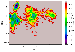
\includegraphics[width=.9\linewidth]{chapter4/2AZC_canc/2AZC_canc-tica.pdf}
  \caption{$2AZC_{canc}-TICA$}
  \label{sup:2AZC_canc-tica}
\end{subfigure}%
\begin{subfigure}{.5\textwidth}
  \centering
  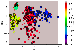
\includegraphics[width=.9\linewidth]{chapter4/2AZC_canc/2AZC_canc-pcca.pdf}
  \caption{$2AZC_{canc}-PCCA$}
  \label{sup:2AZC_canc-pcca}
\end{subfigure}
\caption{PCCA clustering in TICA space from simulations of $2AZC_{canc}$. MD simulations for $2AZC_{canc}$ show sampling of 4 different binding modes (red, yellow, blue, and green), where the dominant binding mode is indicated in red.}
\label{sup:2AZC_canc-cluster}
\end{figure}

\begin{figure}[!ht]
\centering
\begin{subfigure}{.5\textwidth}
  \centering
  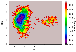
\includegraphics[width=.9\linewidth]{chapter4/2AZU_canc/2AZU_canc-tica.pdf}
  \caption{$2AZU_{canc}-TICA$}
  \label{sup:2AZU_canc-tica}
\end{subfigure}%
\begin{subfigure}{.5\textwidth}
  \centering
  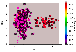
\includegraphics[width=.9\linewidth]{chapter4/2AZU_canc/2AZU_canc-pcca.pdf}
  \caption{$2AZU_{canc}-PCCA$}
  \label{sup:2AZU_canc-pcca}
\end{subfigure}
\caption{PCCA clustering in TICA space from simulations of $2AZU_{canc}$. MD simulations for $2AZU_{canc}$ show sampling of 2 different binding modes (pink and red), where the dominant binding mode is shown in pink.}
\label{sup:2AZU_canc-cluster}
\end{figure}

\begin{figure}[!ht]
\centering
\begin{subfigure}{.5\textwidth}
  \centering
  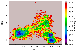
\includegraphics[width=.9\linewidth]{chapter4/2AZC_flip/2AZC_flip-tica.pdf}
  \caption{$2AZC_{flip}-TICA$}
  \label{sup:2AZC_flip-tica}
\end{subfigure}%
\begin{subfigure}{.5\textwidth}
  \centering
  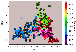
\includegraphics[width=.9\linewidth]{chapter4/2AZC_flip/2AZC_flip-pcca.pdf}
  \caption{$2AZC_{flip}-PCCA$}
  \label{sup:2AZC_flip-pcca}
\end{subfigure}
\caption{PCCA clustering in TICA space from simulations of $2AZC_{flip}$. MD simulations for $2AZC_{flip}$ show sampling of 4 different binding modes (red, pink, blue, and green), where the primary binding mode is indicated in blue.}
\label{sup:2AZC_flip-cluster}
\end{figure}

\begin{figure}[!ht]
\centering
\begin{subfigure}{.5\textwidth}
  \centering
  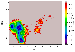
\includegraphics[width=.9\linewidth]{chapter4/2AZU_flip/2AZU_flip-tica.pdf}
  \caption{$2AZU_{flip}-TICA$}
  \label{sup:2AZU_flip-tica}
\end{subfigure}%
\begin{subfigure}{.5\textwidth}
  \centering
  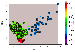
\includegraphics[width=.9\linewidth]{chapter4/2AZU_flip/2AZU_flip-pcca.pdf}
  \caption{$2AZU_{flip}-PCCA$}
  \label{sup:2AZU_flip-pcca}
\end{subfigure}
\caption{PCCA clustering in TICA space from simulations of $2AZU_{flip}$. MD simulations for $2AZU_{flip}$ show sampling of 3 different binding modes (red, blue and green), where the primary binding mode is indicated in green.}
\label{sup:2AZU_flip-cluster}
\end{figure}